Bazujac na pracach numerycznych na jednowymiarowych siatkach dyfrakcyjnych pozwalajachych na wzbudzenie modow falowodowych w podkladach z GaAs przeanalizowane zostalo dzialanie analogicznych falowodow zbudowanych z siatek koncentrycznych. 

Bazujac na analitycznym rozwiazaniu problemu wzbudzania modow falowodowych w podkladzie dielektrycznym (przy zalozeniu nieskonczonych wymiarow w kierunku propagacji wewnatrz falowodu) sporzadzono wykres przedstawiajacy zaleznosc okresu siatki pozwalajacej na wzbudzenie modu falowodowego od dlugosci fali w prozni promieniowania padajacego na uklad.

\begin{figure}
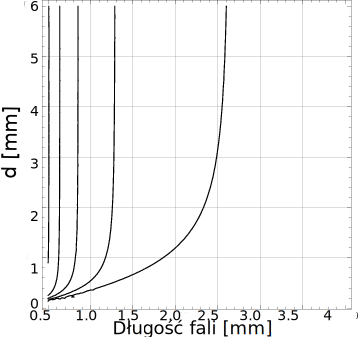
\includegraphics{images/antenaThz/d_lambda.png}
\end{figure}

Wielosc galezi wynika z faktu, ze dla krotszych dlugosci fali rozpatrywany podklad ma charakter wielomodowy. Pojedyncze rozwiazanie powyzej dlugosci fali rownej 3mm, wskazuje nam poczatek zakresu jednomodowego.

\begin{figure}
\includegraphics{images/antenaThz/ro_consrc_radial_antena.png}
\end{figure}

Dla weryfikacji mozliwosci dzialania zaprojektowanych falowodow, przeprowadzono symulacje FDTD we wspolrzednych cylindryczncych. Symulacje potwierdzily mozliwosc wykorzystanie powyzszych siatek zarowno przy oswietleniu ukladu polaryzacja radialna jak  i liniowa. Ponizej przedstawiony rysunek opisuje sytuacje w ktorej struktura z GaAs o rozmiarach 10x10mm pokryta siatka dyfrakcyjna o okresie 538 um i otworach 250um (wspolczynnik wypelnienia ok. 0.53) zostala oswietlona promieniowaniem o dlugosci fali 2.52 mm. W przypadku prezentowanej symulacji siatka miala grubosc 10um, w kolejnych symulacjach potwierdzono jednak, ze grubosc siatki nie ma kluczowego zanczenia pod warunkiem zapewnienia nie przezroczystosci siatki. Efekt koncentracji pola przy zblizaniu sie do srodka struktury wynika ze zmniejszania sie elementu objetosciowego wraz ze zblizaniem do osi symetrii. 



